\section{Incremental queries, change propagation}



\subsection{Rete}


\subsubsection{Detailed Rete with an actual instance model}


\myFigure{rete-routesensor-example-instances}{An instance model of the \tb's metamodel}

\myFigure{rete-routesensor-example-rete}{The Rete net and the partial matches stored in its nodes}



\subsection{Distribution}


\subsubsection{Principles}


\subsubsection{Practice (transparent framework: Akka)}





\emph{Distributed pattern matcher.}\label{distributed_pattern_matcher}
On top of the middleware, \iqd{} constructs a distributed and asynchronous network of communicating nodes that implement the Rete~\cite{Forgy} algorithm (shown within the dashed region in \autoref{fig:architecture}). This layer is essentially a dataflow network, with two types of nodes. Change notification objects (tokens) are propagated to intermediate \emph{worker nodes} that perform operations (like filtering tokens based on constant expressions, or performing join or antijoin operations based on their contents) and
store partial (interim) query results in their own memory. In contrast, \emph{production nodes} are terminators that provide an interface for fetching query results and also their changes. Connections between nodes can be \emph{local} (within one host) or \emph{remote} (when two Rete nodes are allocated to different hosts). It is important to emphasize that the database shards and Rete nodes are two distinct levels of distribution that do not directly depend upon each other.

% \begin{figure}[!h]
% \begin{center}
% \begin{tabular}{cc}
% \begin{minipage}{0.35\columnwidth}
% \begin{lstlisting}
% pattern test(
%   V1:Type1, V2:Type2,
%   V3:Type3, V4:Type4) {
%   Type1.edgeType1(V1, V2);
%   // join 1
%   Type2.edgeType2(V2, V3);
%   // join 2
%   Type3.edgeType3(V3, V4);
%   // antijoin
%   neg find anti(V4, V1);
% }
% pattern anti(V4, V1) {
%  Type1.edgeType4(V4, V1);
% }
% \end{lstlisting}
% \end{minipage}
% \hspace{0.5cm}
% \begin{minipage}{0.45\columnwidth}
%   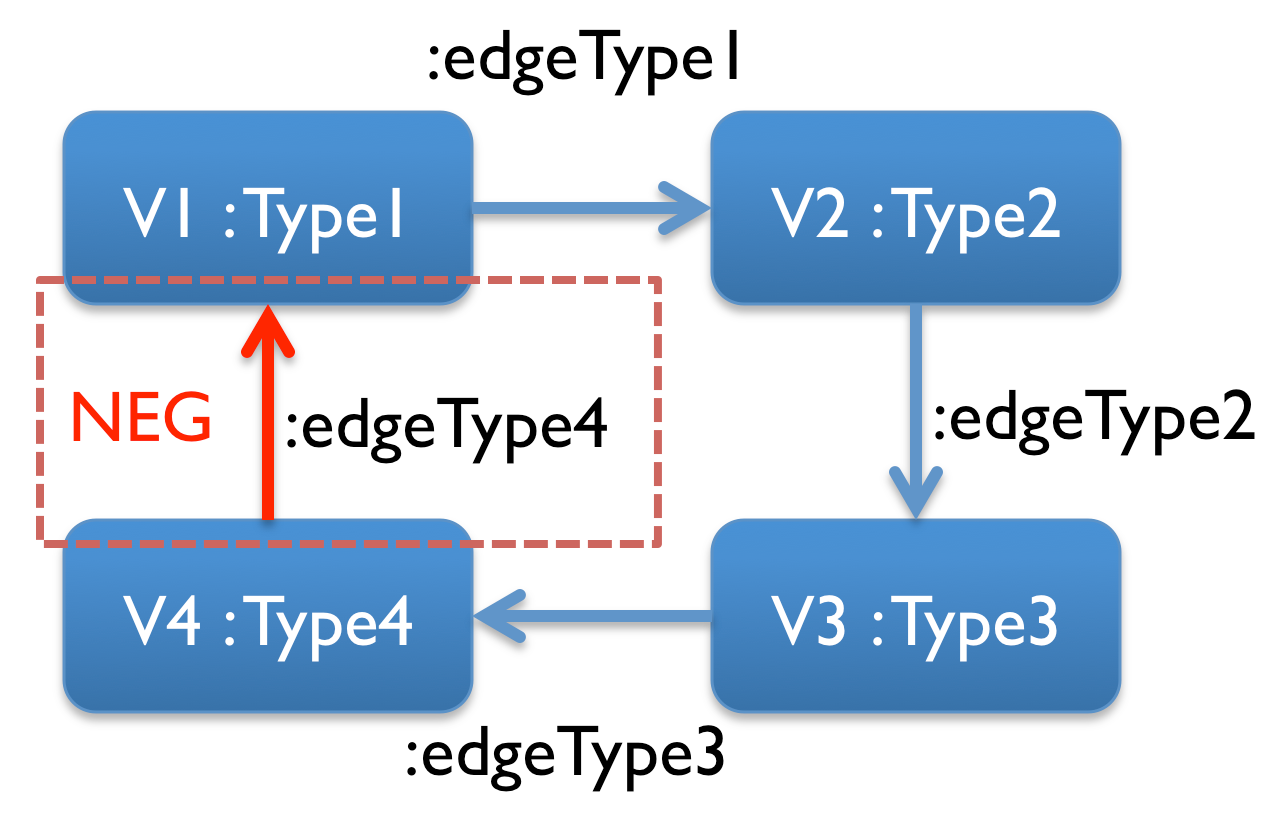
\includegraphics[width=\textwidth]{figures/patterndef}
% \end{minipage}
% \end{tabular}
% \end{center}
% \caption{Example graph query}
% \label{fig:patterndef}
% \end{figure}



\subsection{Scalability considerations}
For the storage layer, the most important issue from an incremental query evaluation perspective is that the indexers of the middleware should be filled as quickly as possible. This favors technologies where model sharding can be performed efficiently (i.e.\ with balanced shards in terms of type-instance relationships), and elementary queries (or model graph traversals) can be executed efficiently.

Achieving scalability of the distributed Rete architecture is an equally complex challenge. The overall performance of the system is influenced by a number of factors, including (i) the \emph{layout of the Rete network} (which can be optimized depending on both query and instance model characteristics, e.g.\ to keep the resource requirement of intermediate join operations to a minimum), (ii) the \emph{allocation} of Rete nodes to host computers (e.g.\ to optimize local resource usage, or to minimize the amount of remote network communication), and (iii) \emph{dynamic adaptability} to changing conditions (e.g.\ when the model size and thus query result size grows rapidly, the Rete network may require dynamic reallocation or node sharding due to local resource limitations).
